\documentclass{article} % say
\usepackage{tikz}
\begin{document}
\begin{center}
%\pgfplotsset{compat=1.18}
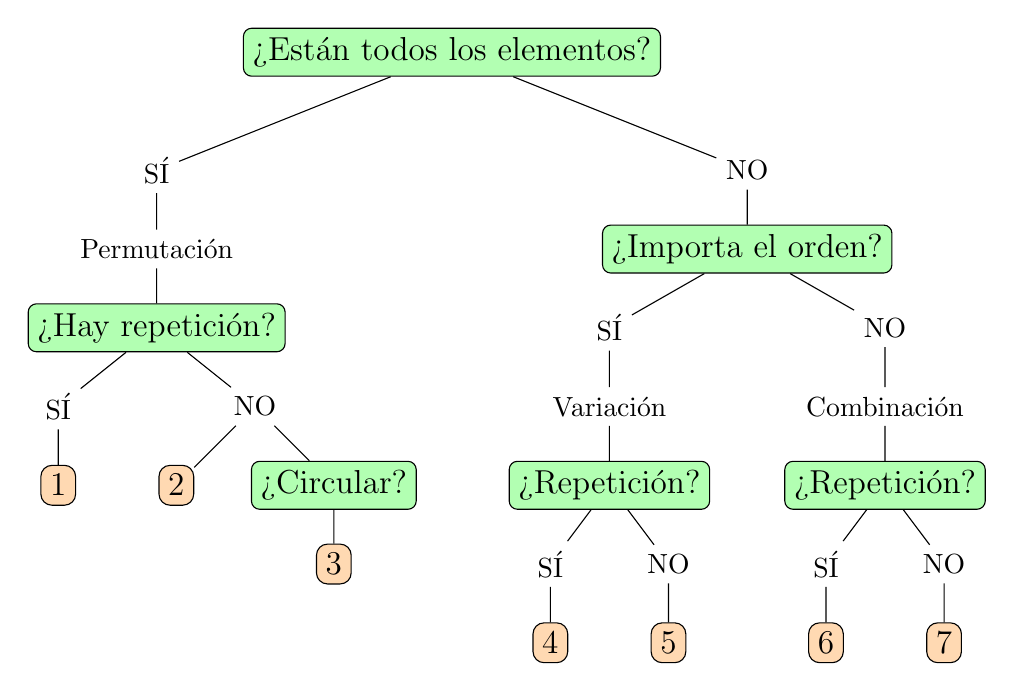
\begin{tikzpicture}
\tikzstyle{level 1} = [sibling distance=7.5cm, level distance=1.5cm]
\tikzstyle{level 2} = [sibling distance=2cm, level distance=1cm]
\tikzstyle{level 3} = [sibling distance=3.5cm, level distance=1cm]
\tikzstyle{level 4} = [sibling distance=2.5cm, level distance=1cm]
\tikzstyle{level 5} = [sibling distance=2cm, level distance=1cm]
\tikzstyle{level 6} = [sibling distance=1.5cm, level distance=1cm]
\tikzstyle{arestas}=[rectangle,rounded corners=4pt,fill=orange!30,draw=black,font=\large]
\tikzstyle{berdex}=[rectangle,rounded corners=3pt,fill=green!30,draw=black,font=\large]
\node[berdex]{¿Están todos los elementos?}
child{
node{SÍ}
    child{
    node{Permutación}
        child{
        node[berdex]{¿Hay repetición?}
            child{
            node{SÍ}
                child{
				        node[arestas]{1}
				        }
            }
            child{
            node{NO}
                child{
				        node[arestas]{2}
                }
				        child{
				        node[berdex]{¿Circular?}
				            child{
				            node[arestas]{3}
				            }
                }   
            }
        }
    }
}
child{
node{NO}
    child{
    node[berdex]{¿Importa el orden?}
        child{
        node{SÍ}
            child{
            node{Variación}
                child{
                node[berdex]{¿Repetición?}
                    child{
                    node{SÍ}
                        child{
				                node[arestas]{4}
				                }
                    }
                    child{
                    node{NO}
                        child{
				                node[arestas]{5}
				                }
                    }
                }
            }
        }
        child{
        node{NO}
            child{
            node{Combinación}
                child{
                node[berdex]{¿Repetición?}
                    child{
                    node{SÍ}
                        child{
				                node[arestas]{6}
				                }
                    }
                    child{
                    node{NO}
                        child{
				                node[arestas]{7}
				                }
                    }
                }
            }
        }
    }    
};
\end{tikzpicture}   
\end{center}
\end{document}
